\documentclass[10pt,xcolor={table,xcdraw}]{beamer}
\usetheme[
%%% options passed to the outer theme
%    hidetitle,           % hide the (short) title in the sidebar
%    hideauthor,          % hide the (short) author in the sidebar
%    hideinstitute,       % hide the (short) institute in the bottom of the sidebar
%    shownavsym,       \usepackage[table,xcdraw]{xcolor}   % show the navigation symbols
%    width=2cm,           % width of the sidebar (default is 2 cm)
    hideothersubsections,% hide all subsections but the subsections in the current section
%    hideallsubsections,  % hide all subsections
    left               % right of left position of sidebar (default is right)
%%% options passed to the color theme
%    lightheaderbg,       % use a light header background
  ]{AAUsidebar}

% If you want to change the colors of the various elements in the theme, edit and uncomment the following lines
% Change the bar and sidebar colors:
%\setbeamercolor{AAUsidebar}{fg=red!20,bg=red}
%\setbeamercolor{sidebar}{bg=red!20}
% Change the color of the structural elements:
%\setbeamercolor{structure}{fg=red}
% Change the frame title text color:
%\setbeamercolor{frametitle}{fg=blue}
% Change the normal text color background:
%\setbeamercolor{normal text}{bg=gray!10}
% ... and you can of course change a lot more - see the beamer user manual.
\usepackage{mdframed}
\usepackage[utf8]{inputenc}
\usepackage[english]{babel}
\usepackage[T1]{fontenc}
% Or whatever. Note that the encoding and the font should match. If T1
% does not look nice, try deleting the line with the fontenc.
\usepackage{helvet}

% colored hyperlinks
\newcommand{\chref}[2]{%
  \href{#1}{{\usebeamercolor[bg]{AAUsidebar}#2}}%
}

\title[Report Presentation]% optional, use only with long paper titles
{A Game of Paradigms}
\subtitle{A Usability Study of Functional Idioms in Gameplay Programming}  % could also be a conference name

\date{}%\today}

\author[Thomas Gwynfryn McCollin \and Tobias Morell] % optional, use only with lots of authors
{}
% - Give the names in the same order as they appear in the paper.
% - Use the \inst{?} command only if the authors have different
%   affiliation. See the beamer manual for an example

\institute[
%  {\includegraphics[scale=0.2]{aau_segl}}\\ %insert a company, department or university logo
  Dept.\ of Computer Science\\
  Aalborg University\\

] % optional - is placed in the bottom of the sidebar on every slide
{% is placed on the title page
  Department of Computer Science\\
  Aalborg University\\
  Denmark

  %there must be an empty line above this line - otherwise some unwanted space is added between the university and the country (I do not know why;( )
}


% specify a logo on the titlepage (you can specify additional logos an include them in
% institute command below
\pgfdeclareimage[height=1.5cm]{titlepagelogo}{AAUgraphics/aau_logo_new} % placed on the title page
%\pgfdeclareimage[height=1.5cm]{titlepagelogo2}{graphics/aau_logo_new} % placed on the title page
\titlegraphic{% is placed on the bottom of the title page
  \pgfuseimage{titlepagelogo}
%  \hspace{1cm}\pgfuseimage{titlepagelogo2}
}

\newcommand{\projectFullTitle}{\projectTitle : \projectSubtitle}
\newcommand{\projectTitle}{Battle of Languages}
\newcommand{\projectSubtitle}{C\# vs. F\#}
\newcommand{\group}{PT103F19}
%%%%%%%%%%%%%%%%%%%%%%%%%%%%%%%%%%%%%%%%%%%%%%%%
% Language, Encoding and Fonts
% http://en.wikibooks.org/wiki/LaTeX/Internationalization
%%%%%%%%%%%%%%%%%%%%%%%%%%%%%%%%%%%%%%%%%%%%%%%%
% Select encoding of your inputs. Depends on
% your operating system and its default input
% encoding. Typically, you should use
%   Linux  : utf8 (most modern Linux distributions)
%            latin1
%   Windows: ansinew
%            latin1 (works in most cases)
%   Mac    : applemac
% Notice that you can manually change the input
% encoding of your files by selecting "save as"
% an select the desired input encoding.
\usepackage{scrextend}
\usepackage[utf8]{inputenc}
\usepackage[nointegrals]{wasysym}
%\usepackage{float}
\usepackage{xspace}
\usepackage{floatrow}
\usepackage{booktabs}
\usepackage{multicol}

\usepackage{siunitx}
\usepackage{csvsimple}
\usepackage[table,xcdraw]{xcolor}
% Make latex understand and use the typographic
% rules of the language used in the document.
\usepackage{array}
\usepackage[english]{babel}
% Use the vector font Latin Modern which is going
% to be the default font in latex in the future.
\usepackage{lmodern}
% Choose the font encoding
\usepackage[T1]{fontenc}
\usepackage{lastpage} % Tilføjet af Jesper, får sidetal til at virke.
%%%%%%%%%%%%%%%%%%%%%%%%%%%%%%%%%%%%%%%%%%%%%%%%
% Graphics and Tables
% http://en.wikibooks.org/wiki/LaTeX/Importing_Graphics
% http://en.wikibooks.org/wiki/LaTeX/Tables
% http://en.wikibooks.org/wiki/LaTeX/Colors
%%%%%%%%%%%%%%%%%%%%%%%%%%%%%%%%%%%%%%%%%%%%%%%%
% load a colour package
\usepackage[table]{xcolor}

\definecolor{aaublue}{RGB}{33,26,82}% dark blue
\definecolor{editgreen}{HTML}{008000}% dark green
% The standard graphics inclusion package
\usepackage{graphicx}
% Set up how figure and table captions are displayed
\usepackage[within=none]{caption}
\captionsetup{%
  font=footnotesize,% set font size to footnotesize
  labelfont=bf % bold label (e.g., Figure 3.2) font
}
% Make the standard latex tables look so much better
\usepackage{array,booktabs}
% Enable the use of frames around, e.g., theorems
% The framed package is used in the example environment
\usepackage{framed}

\usepackage{pgfplots}
\usepackage{pgfplotstable}
\pgfplotsset{compat=1.15}
\usepackage{tikz}
\usetikzlibrary{arrows,arrows.meta, fit, backgrounds, positioning, automata, shapes}
\usepackage{enumitem}
%%%%%%%%%%%%%%%%%%%%%%%%%%%%%%%%%%%%%%%%%%%%%%%%
% Mathematics
% http://en.wikibooks.org/wiki/LaTeX/Mathematics
%%%%%%%%%%%%%%%%%%%%%%%%%%%%%%%%%%%%%%%%%%%%%%%%
% Defines new environments such as equation,
% align and split
\usepackage{amsmath}
% Adds new math symbols
\usepackage{amssymb}
% Use theorems in your document
% The ntheorem package is also used for the example environment
% When using thmmarks, amsmath must be an option as well. Otherwise \eqref doesn't work anymore.
\usepackage[framed,amsmath,thmmarks]{ntheorem}

%%%%%%%%%%%%%%%%%%%%%%%%%%%%%%%%%%%%%%%%%%%%%%%%
% Page Layout
% http://en.wikibooks.org/wiki/LaTeX/Page_Layout
%%%%%%%%%%%%%%%%%%%%%%%%%%%%%%%%%%%%%%%%%%%%%%%%
% Change margins, papersize, etc of the document
\usepackage[top=1in, bottom=1.5in]{geometry}%, left=1in, right=1in]{geometry}

\setlength\parindent{0pt}   % Remove paragraph indentation
\setlength\parskip{1em}     % Sets paragraph spacing
%\usepackage[
%  inner=28mm,% left margin on an odd page
%  outer=41mm,% right margin on an odd page
%  ]{geometry}
% Modify how \chapter, \section, etc. look
% The titlesec package is very configureable

%%%%% Titles and sections
\usepackage{titlesec}
\newcommand{\hsp}{\hspace{20pt}}
\titleformat{\chapter}[hang]{\Huge\bfseries}{\thechapter\hsp|\hsp}{0pt}{}[]
\titleformat*{\section}{\normalfont\Large\bfseries}
\titleformat*{\subsection}{\normalfont\large\bfseries}
\titleformat*{\subsubsection}{\normalfont\normalsize\bfseries}

\titlespacing*{\chapter}{0pt}{0.5cm}{1cm}
\titlespacing*{name=\chapter,numberless}{0pt}{0.5cm}{1cm}

% Clear empty pages between chapters
\let\origdoublepage\cleardoublepage
\newcommand{\clearemptydoublepage}{%
  \clearpage
  {\pagestyle{empty}\origdoublepage}%
}
\let\cleardoublepage\clearemptydoublepage

% Change the headers and footers
\usepackage{fancyhdr}
\pagestyle{fancy}
\fancyhf{} %delete everything
\renewcommand{\headrulewidth}{0pt} %remove the horizontal line in the header
\fancyfoot[C]{\thepage} %page number on all pages
\setlength{\headheight}{14pt}
% Do not stretch the content of a page. Instead,
% insert white space at the bottom of the page
\raggedbottom
% Enable arithmetics with length. Useful when
% typesetting the layout.
\usepackage{calc}

\usepackage[
%  disable, %turn off todonotes
  colorinlistoftodos, %enable a coloured square in the list of todos
  textwidth=1.1\marginparwidth, %set the width of the todonotes
  textsize=scriptsize, %size of the text in the todonotes
  ]{todonotes}

\usepackage[T1]{fontenc}
\usepackage{inconsolata}
\usepackage{color}
\usepackage{svg}

\usepackage{listings}
% see, e.g., http://en.wikibooks.org/wiki/LaTeX/Customizing_LaTeX#New_commands
% for more information on how to create macros

%%%%%%%%%%%%%%%%%%%%%%%%%%%%%%%%%%%%%%%%%%%%%%%%
% Macros for the titlepage
%%%%%%%%%%%%%%%%%%%%%%%%%%%%%%%%%%%%%%%%%%%%%%%%
%Creates the aau titlepage
\newcommand{\aautitlepage}[3]{%
  {
    %set up various length
    \ifx\titlepageleftcolumnwidth\undefined
      \newlength{\titlepageleftcolumnwidth}
      \newlength{\titlepagerightcolumnwidth}
    \fi
    \setlength{\titlepageleftcolumnwidth}{0.5\textwidth-\tabcolsep}
    \setlength{\titlepagerightcolumnwidth}{\textwidth-2\tabcolsep-\titlepageleftcolumnwidth}
    %create title page
    \thispagestyle{empty}
    \noindent%
    \begin{tabular}{@{}ll@{}}
      \parbox{\titlepageleftcolumnwidth}{
        \iflanguage{danish}{%
          \includegraphics[width=\titlepageleftcolumnwidth]{00-images/aau-logo-da}
        }{%
          
\includegraphics[width=\titlepageleftcolumnwidth]{00-images/aau-logo-en}
        }
      } &
      \parbox{\titlepagerightcolumnwidth}{\raggedleft\sf\small
        #2
      }\bigskip\\
       #1 &
      \parbox[t]{\titlepagerightcolumnwidth}{%
      \textbf{Abstract:}\bigskip\par
        \fbox{\parbox{\titlepagerightcolumnwidth-2\fboxsep-2\fboxrule}{%
          #3
        }}
      }\\
    \end{tabular}
    \vfill
    \iflanguage{danish}{%
      \noindent{\footnotesize\emph{Rapportens indhold er frit tilgængeligt, men offentliggørelse (med kildeangivelse) må kun ske efter aftale med forfatterne.}}
    }{%
      \noindent{\footnotesize\emph{The content of this report is freely available, but publication (with reference) may only be pursued due to agreement with the author.}}
    }
    \clearpage
  }
}

%Create english project info
\newcommand{\englishprojectinfo}[8]{%
  \parbox[t]{\titlepageleftcolumnwidth}{
    \textbf{Title:}\\ #1\bigskip\par
    \textbf{Theme:}\\ #2\bigskip\par
    \textbf{Project Period:}\\ #3\bigskip\par
    \textbf{Project Group:}\\ #4\bigskip\par
    \textbf{Participant(s):}\\ #5\bigskip\par
    \textbf{Supervisor(s):}\\ #6\bigskip\par
    \textbf{Copies:} #7\bigskip\par
    \textbf{Page Numbers:} \pageref{LastPage}\bigskip\par
    \textbf{Date of Completion:}\\ #8
  }
}

%Create danish project info
\newcommand{\danishprojectinfo}[8]{%
  \parbox[t]{\titlepageleftcolumnwidth}{
    \textbf{Titel:}\\ #1\bigskip\par
    \textbf{Tema:}\\ #2\bigskip\par
    \textbf{Projektperiode:}\\ #3\bigskip\par
    \textbf{Projektgruppe:}\\ #4\bigskip\par
    \textbf{Deltagere:}\\ #5\bigskip\par
    \textbf{Vejleder:}\\ #6\bigskip\par
    \textbf{Oplagstal:} #7\bigskip\par
    \textbf{Sidetal:} \pageref{LastPage}\bigskip\par
    \textbf{Afleveringsdato:}\\ #8
  }
}

\usepackage{courier}
\definecolor{gray}{rgb}{0.4,0.4,0.4}
\definecolor{darkblue}{rgb}{0.0,0.0,0.6}
\definecolor{cyan}{rgb}{0.0,0.6,0.6}


%\setmonofont{Consolas} %to be used with XeLaTeX or LuaLaTeX
\definecolor{bluekeywords}{rgb}{0,0,1}
\definecolor{greencomments}{rgb}{0,0.5,0}
\definecolor{redstrings}{rgb}{0.64,0.08,0.08}
\definecolor{xmlcomments}{rgb}{0.5,0.5,0.5}
\definecolor{types}{rgb}{0.17,0.57,0.68}

\usepackage{hyperref}
\hypersetup{%
	plainpages=false,%
	pdfauthor={PT902E18 - Tobias Morell, Thomas Gwynfryn McCollin},%
	pdftitle={P9},%
	pdfsubject={Project Report},%
	bookmarksnumbered=true,%
	colorlinks,%
	citecolor=aaublue,%
	filecolor=aaublue,%
	linkcolor=aaublue,% you should probably change this to black before printing
	urlcolor=aaublue,%
	pdfstartview=FitH%
}
% PDF package
\usepackage[final]{pdfpages}
\usepackage{glossaries}
\usepackage{longtable}
\usepackage{tasks}
\usepackage{subcaption}
\usepackage{setspace}
\addtokomafont{labelinglabel}{\sffamily\bfseries}
\usepackage{dirtytalk}
\usepackage{etoolbox}
\usepackage{silence}

\usepackage[backend=biber, style=ieee, urldate=long]{biblatex} % biblatex - bibliography tool %
\bibliography{00-preliminary/bib}
\renewcommand*{\lstlistlistingname}{List of Listings}

\setlength{\headheight}{15pt}

\usepackage{rotating}
\usepackage{tablefootnote}

% Style to select only points from #1 to #2 (inclusive)
\pgfplotsset{select coords between index/.style 2 args={
    x filter/.code={
        \ifnum\coordindex<#1\def\pgfmathresult{}\fi
        \ifnum\coordindex>#2\def\pgfmathresult{}\fi
    }
}}

\usepackage[outputdir=build]{minted}
%%%%%%%%%% C# %%%%%%%%%%
\setminted[csharp]{
frame=single,%lines
framesep=2mm,
fontsize=\footnotesize,
linenos,
breaklines
}
\usemintedstyle[csharp]{vs}

\setminted[fsharp]{
frame=single,%lines
framesep=2mm,
fontsize=\footnotesize,
linenos,
breaklines
}
\usemintedstyle[fsharp]{vs}

% Quotations package
\usepackage[autostyle]{csquotes}

%%%%%%%%%%%%%%%%%%% Packages %%%%%%%%%%%%%%%%%%%
\usepackage{xifthen}
\usepackage{xparse}


%%%%%%%%%%%%%%%%%%% PGF Styles%%%%%%%%%%%%%%%%%%%
\pgfplotsset{
  abs log x ticks/.style={
      xticklabel={
        \pgfkeys{/pgf/fpu=true}
        \pgfmathparse{exp(\tick)}%
        \pgfmathprintnumber[fixed relative, precision=3]{\pgfmathresult}
        \pgfkeys{/pgf/fpu=false}
      }
  },
  abs log y ticks/.style={
      yticklabel={
        \pgfkeys{/pgf/fpu=true}
        \pgfmathparse{exp(\tick)}%
        \pgfmathprintnumber[fixed relative, precision=3]{\pgfmathresult}
        \pgfkeys{/pgf/fpu=false}
      }
  }
}

%%%%%%%%%%%%%%%%%%% Commands %%%%%%%%%%%%%%%%%%%
\newcommand{\ifequals}[3]{\ifthenelse{\equal{#1}{#2}}{#3}{}}
\newcommand{\case}[2]{#1 #2} % Dummy, so \renewcommand has something to overwrite...
\newenvironment{switch}[1]{\renewcommand{\case}{\ifequals{#1}}}{}

\newcommand{\symbolicsStrat}{%
symbolic x coords={,
    Problem,
    10,
    100,
    1000,
    10000,
    100000,
}
}

\newcommand{\symbolic}[1]{symbolic x coords={#1}}
\NewDocumentCommand\lnm{O{y}O{2}}{%
\begin{switch}{#1}%
    \case{x}{xmode=log, log basis x={#2}}%
    \case{y}{ymode=log, log basis y={#2}}%
\end{switch}%
}
\newcommand{\plotData}[2]{
    \addplot table [y={#1}] {#2};
    \addlegendentry{#1};
}

\newcommand{\plotUnmarkedData}[2]{
  \addplot+[mark=none] table [y={#1}] {#2};
  \addlegendentry{#1};
}

\NewDocumentCommand\optPlotData{O{}mm}{
  \addplot+[#1] table [y={#2}] {#3};
  \addlegendentry{#2};
}

\newcommand{\plotDataWithError}[2]{
    \addplot+[error bars/.cd, y dir=both,y explicit] table [y={#1}, y error={#1 Error}] {#2};
    \addlegendentry{#1};
}

\newcommand{\plotDataWithErrorAndLegend}[3]{
    \addplot+[error bars/.cd, y dir=both,y explicit] table [y={#1}, y error={#1 Error}] {#2};
    \addlegendentry{#3};
}

\newcommand{\logmode}[1]{\IfBooleanTF{#1}{log}{normal}}
\newcommand{\logbase}[1]{\IfBooleanTF{#1}{2}{1}}

% O/o for optional, M/m for mandatory, s for star
% s #1 BooleanTrue if star, BooleanFalse otherwise
% O #2 PGFPlot options
% O #3 Y label
% O #4 X label
% m #5 Caption
% m #6 Label
% m #7 Plots
\NewDocumentCommand\lineChart{sO{}O{Logarithmic Run Time (ns)}O{Lower is better}mmm}{%

\begin{figure}[H]
\makebox[\textwidth][c]{
\tikzsetnextfilename{#6}
\begin{tikzpicture}
    \begin{axis}[
        ylabel={#3},
        xlabel={#4},
        width=1.2\textwidth,
        height=8cm,
        ymajorgrids,
        xtick=data,
        #2,
        ymode/.expand once=\logmode{#1},
        log basis y/.expand once=\logbase{#1},
        xticklabel style={rotate=45, anchor=east},
        legend columns = -1,
        legend style={
            draw=none,
            at={(0.5,1.05)},
            anchor=south,
            column sep=1ex,
            font=\tiny
        }
    ]
    #7
    \end{axis}
\end{tikzpicture}}
\caption{#5}
\label{fig:#6}
\end{figure}
}

% O/o for optional, M/m for mandatory, s for star
% s #1 BooleanTrue if star, BooleanFalse otherwise
% O #2 bar width
% O #3 PGFPlot options
% O #4 Y label
% O #5 X label
% m #6 Caption
% m #7 Label
% m #8 Plots
\NewDocumentCommand\barChart{sO{12}O{}O{Run Time (ns)}O{Lower is better}mmm}{%
    \begin{figure}[H]
    \makebox[\textwidth][c]{
    \tikzsetnextfilename{#7}
    \begin{tikzpicture}
        \begin{axis}[
            ylabel={#4},
            xlabel={#5},
            width=1.2\textwidth,
            height=8cm,
            ymajorgrids,
            xtick=data,
            ybar=0.4pt,
            bar width=#2pt,
            xticklabel style={rotate=45, anchor=east},
            #3,
            ymode/.expand once=\logmode{#1},
            log basis y/.expand once=\logbase{#1},
            legend columns = -1,
            legend style={
                draw=none,
                at={(0.5,1.05)},
                anchor=south,
                column sep=1ex,
                font=\tiny
            }
        ]
        #8
        \end{axis}
    \end{tikzpicture}}
    \caption{#6}
    \label{fig:#7}
\end{figure}
}


\pgfplotstableread[col sep = comma]{00-data/accumulation.csv}\accumulationData
\pgfplotstableread[col sep = comma]{00-data/summation.csv}\summationData
\pgfplotstableread[col sep = comma]{00-data/work-bias-wait-after-join.csv}\workWithDependencyData
\pgfplotstableread[col sep = comma]{00-data/work-bias-wait-before-join.csv}\workWithoutDependencyData
\pgfplotstableread[col sep =
comma]{00-data/nary-work-bias-wait-after-join.csv}\workWithDependencyDataNary
\pgfplotstableread[col sep =
comma]{00-data/nary-work-bias-wait-before-join.csv}\workWithoutDependencyDataNary
\pgfplotstableread[col sep =
comma]{00-data/linpack.csv}\linpackData
\pgfplotstableread[col sep = comma]{00-data/ai-benchmark-runtimes.csv}\aiBenchmarkRuntimesData
\pgfplotstableread[col sep = comma]{00-data/ai-benchmark.csv}\aiBenchmarkData
\pgfplotstableread[col sep = comma]{00-data/csharp-vs-frp.csv}\aiBenchmarkOverheadData
\pgfplotstableread[col sep = comma]{00-data/csharp-incremental-vs-normal.csv}\aiBenchmarkCsharpGCData
\pgfplotstableread[col sep = comma]{00-data/frp-incremental-vs-normal.csv}\aiBenchmarkFsharpGCData


%%%%%%%% Beamer Bullshit %%%%%%%%
\newenvironment{changemargin}[2]{%
  \begin{list}{}{%
    \setlength{\topsep}{0pt}%
    \setlength{\leftmargin}{#1}%
    \setlength{\rightmargin}{#2}%
    \setlength{\listparindent}{\parindent}%
    \setlength{\itemindent}{\parindent}%
    \setlength{\parsep}{\parskip}%
  }%
  \item[]}{\end{list}}

\begin{document}
\begin{frame}[plain,noframenumbering]
  \begin{changemargin}{-1.6cm}{0cm}
  \begin{center}
  \begin{figure}[H]
      \includesvg[height=.6\textheight]{../00-images/battle-of-langs}
      \caption{Made using icons by \href{https://www.freepik.com/}{Freepik} and \href{https://www.flaticon.com/authors/nikita-golubev}{Nikita Golubev} from \href{https://www.flaticon.com/}{\color{blue}www.flaticon.com}}
  \end{figure}
  \end{center}
  \end{changemargin}
\end{frame}
% the titlepage
{\aauwavesbg%
\begin{frame}[plain,noframenumbering] % the plain option removes the sidebar and header from the title page
  \titlepage
\end{frame}}
%%%%%%%%%%%%%%%%

% TOC
\section{Backgound}\label{sec:background}
\begin{frame}{\nameref{sec:background}}{Table of Contents}
{\footnotesize
\tableofcontents[hideothersubsections]}
\end{frame}
%%%%%%%%%%%%%%%%

\section{Performance Benchmarking}
\begin{frame}{\secname}{Disposition}
	Disposition
    \begin{itemize}
        \item Report Summary
        \item Concurrent Unit Management Benchmark
	\end{itemize}
\end{frame}

\subsection{Report Summary}\label{sec:authors}
\begin{frame}{\secname}{\subsecname}
	.NET Concurrency
	\begin{itemize}
		\item Lenient mapping to Async Workflows and \texttt{Task}s %up to speed?
		\item Sequential code faster in binary tree benchmarks
		\item Concurrent code faster with larger problem sizes:
		\begin{itemize}
			\item 11000 IL instructions in binary tree with no data dependency
			\item 44000 IL instructions in binary tree with data dependency
			\item Column sizes of 512 in matrix summation
		\end{itemize}
		\item Async Workflow concurrency is fragile
	\end{itemize}
\end{frame}

\begin{frame}{\secname}{\subsecname}
	Unity Technologies advices against functional coding style
	\begin{itemize}
		\item High order functions
		\item Closures
		\item Manipulate existing collections rather than mapping
	\end{itemize}
\end{frame}

\begin{frame}{\secname}{\subsecname}
	Unity Performance - What is Unit Management?
	\inlineMovie[loop&autostart]{very-short.avi}{pictures/rts-screenshot.png}{width=\textwidth}
	%\inlineMovie[loop&autostart]{pictures/unit-management-demo.avi}{pictures/rts-screenshot.png}{width=\textwidth}
	% \begin{figure}[h!]
  %       \centering
  %       \includegraphics[width=\textwidth]{pictures/rts-screenshot.png}
  %       \caption{Screenshot from Unit Management scene.}
  %   \end{figure}
\end{frame}

% \fullFrameMovie[loop&autostart]{unit-management-demo.avi}{pictures/rts-screenshot.png}{width=\textwidth}

\begin{frame}{\secname}{\subsecname}
	Unit Management Benchmark
	\begin{itemize}
		\item F\# is marginally slower than C\# in Unity (5-7\%, \cite{maggiore2012formal,bolhuis2019gameplay})
		\item FRP system introduces per-\texttt{GameObject} overhead
	\end{itemize}
\end{frame}

\begin{frame}{\secname}{\subsecname}
	Incorrect Code in Inverse Implementation of Unit Management Benchmark
	\begin{itemize}
		\item State machine has a list of units.
		\item When a unit collides with a shot, the unit is added to the list again.
		\item Many units =\textgreater\ many collisions =\textgreater\ performance degradation
	\end{itemize}
\end{frame}

\begin{frame}[fragile]{\secname}{\subsecname}
	Comparison of Incorrect and Correct Implementation
	\barChart[12][\symbolic{Strategy,500,1000,1500,2000,2500}, width=\textwidth,height=.5\textheight][Average FPS][Number of Units]{Comparison of Correct and Incorrect implementation of Unit Management benchmark using the Mono runtime (higher is better).}{ai:benchmark}{
		\plotData{CSharp Correct}{\sequentialAverageData}
		\plotData{CSharp Incorrect}{\sequentialAverageData}
	}
\end{frame}

\subsection{Concurrent Unit Management Benchmark}

\begin{frame}{\secname}{\subsecname}
	Unity Concurrency Terminology
	\begin{itemize}
		\item \texttt{Job} = A definition of how to update a single entity out of a collection. Jobs are executed on worker threads and may be batched.
		\item \texttt{JobSystem} = A \ttt{MonoBehaviour}, which is in charge of creating and scheduling \texttt{Job}s.
	\end{itemize}
\end{frame}

\begin{frame}{\secname}{\subsecname}
	Setup
	\begin{itemize}
		\item Examine if a concurrent implementation of inverse state machine is faster than sequential
		\item Four \ttt{JobSystem}s:
		\begin{itemize}
			\item Moving Bullets forward
			\item Updating each of the three states (moving, fleeing \& attacking)
		\end{itemize}
		\item Moving between states sequentially
		\item Measure the frame rate over 900 frames
	\end{itemize}
\end{frame}

\begin{frame}{\secname}{\subsecname}
	Setup - Sequential
	\begin{figure}[h!]
        \centering
        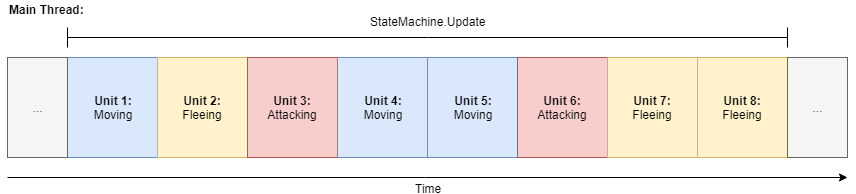
\includegraphics[width=\textwidth]{pictures/sequential.png}
        \caption{A model of sequential execution of inverse state machine.}
    \end{figure}
\end{frame}

\begin{frame}{\secname}{\subsecname}
	Setup - Concurrent
	\begin{figure}[h!]
        \centering
        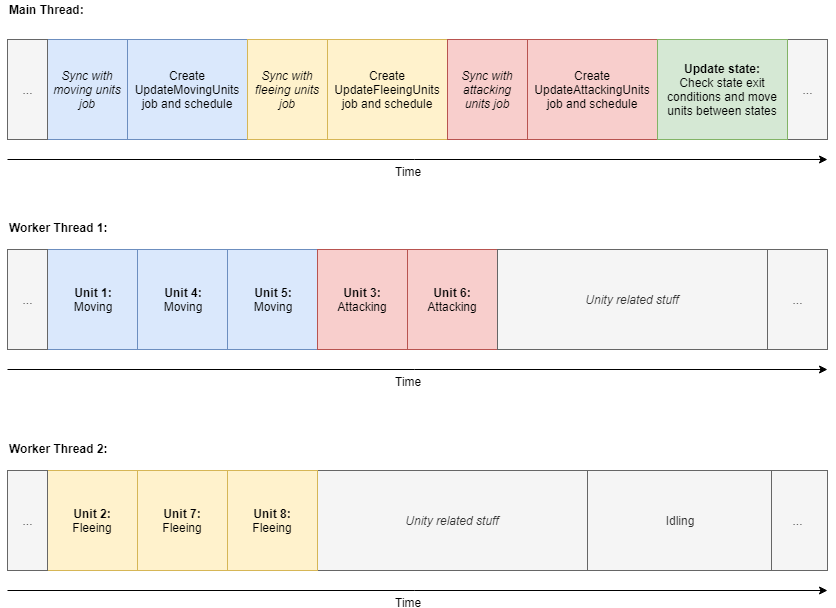
\includegraphics[width=.7\textwidth]{pictures/concurrent.png}
        \caption{A model of concurrent execution of inverse state machine.}
    \end{figure}
\end{frame}

\begin{frame}[fragile]{\secname}{\subsecname}
	Setup - Converting from \ttt{JobSystem} representation to \ttt{Job} representation
	\begin{itemize}
		\item \ttt{JobSystem}s store units (and similar data) in lists
		\item \ttt{Job}s only accept value-type data collections in a \ttt{NativeContainer} (e.g. \ttt{NativeArray})
		\item Units are class instances, i.e. reference
		\item We need to map from a list of references to an array of value-types
	\end{itemize}
\csinline{new TransformAccessArray(}
\csinline{	units.Select(u => u.transform).ToArray(),}
\csinline{	Allocation.TempJob)}
\end{frame}

\begin{frame}{\secname}{\subsecname}
	Setup - Converting from \ttt{JobSystem} representation to \ttt{Job} representation
	\begin{figure}[h!]
        \centering
        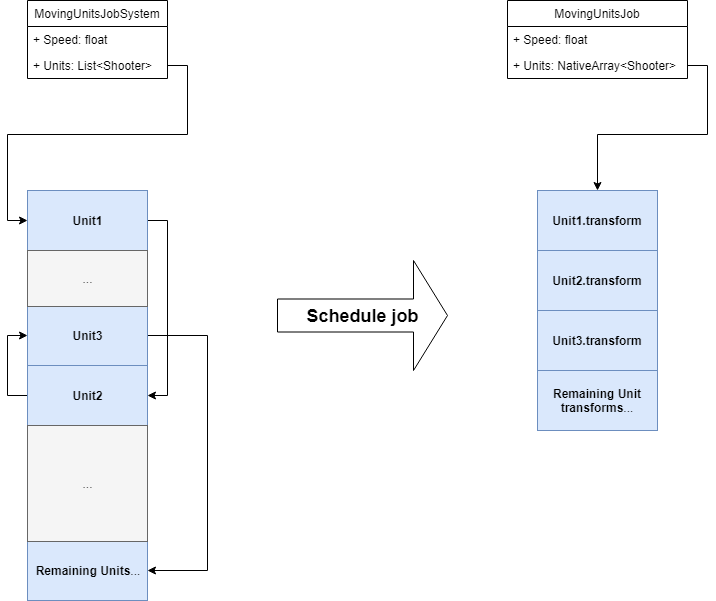
\includegraphics[width=.7\textwidth]{pictures/concurrent-memory-layout.png}
        \caption{Mapping from list of references to array of value-types.}
    \end{figure}
\end{frame}

\begin{frame}{\secname}{\subsecname}
	Setup - Test Machine
	\makeTable{{| l | R{6em} | p{3em} |}
	\hline
	\multicolumn{3}{| c |}{\textbf{Processor}} \\ \hline
	Model & \multicolumn{2}{| c |}{Intel Core i7 4702HQ} \\ \hline
	Clock Frequency & 2.2 & GHz \\ \hline
	Max Turbo & 3.2 & GHz \\ \hline
	Physical & 4 & Cores \\ \hline
	Logical & 8 & Cores \\ \hline
	\multicolumn{3}{|c|}{\textbf{Memory}} \\ \hline
	Memory Size & 16 & GiB  \\ \hline
	Memory Speed & 1600 & MHz \\ \hline
	Memory Type &  \multicolumn{2}{| c |}{DDR3L 1600} \\ \hline
	\multicolumn{3}{|c|}{\textbf{Software}} \\ \hline
	Operating System & \multicolumn{2}{| c |}{Ubuntu 18.04 64bit}  \\ \hline
	C\# runtime & \multicolumn{2}{| c |}{dotnet 2.2.104} \\ \hline
	}{System specifications of the test machine.}{sys-specs}
\end{frame}

\begin{frame}{\secname}{\subsecname}
	Results
	\begin{itemize}
		\item On average roughly equivalent
		\item Sometimes sequential is slower, sometimes not
		\item Concurrent uses a bit more memory (1500 units):
		\begin{itemize}
			\item Sequential: 1.27Gb
			\item Concurrent: 1.36Gb
		\end{itemize}
	\end{itemize}
\end{frame}

\begin{frame}[fragile]{\secname}{\subsecname}
	Average frame rate over 900 frames
	\barChart[12][\symbolic{Strategy,500,1000,1500,2000,2500}, width=\textwidth, height=.5\textheight][Average FPS][Number of Units]{Average frame rate in the sequential and concurrent implementation of Unit Management (higher is better).}{ai:benchmark:avg}{
		\plotData{Sequential}{\aiAverageData}
		\plotData{Concurrent}{\aiAverageData}
	}
\end{frame}

\begin{frame}[fragile]{\secname}{\subsecname}
	\lineChart[enlarge x limits=false, width=\textwidth, height=.6\textheight, xtick={100,200,300,400,500,600,700,800}][FPS][Frame No.]{FPS for each frame with 500 units (higher is better).}{ai:benchmark:500}{
    \plotUnmarkedData{Sequential 500}{\sequentialData}
    \plotUnmarkedData{Concurrent 500}{\concurrentData}
}
\end{frame}

\iffalse
\begin{frame}[fragile]{\secname}{\subsecname}
	\lineChart[enlarge x limits=false, width=\textwidth, height=.6\textheight, xtick={100,200,300,400,500,600,700,800}][FPS][Frame No.]{FPS for each frame with 1000 units (higher is better).}{ai:benchmark:1000}{
    \plotUnmarkedData{Sequential 1000}{\sequentialData}
    \plotUnmarkedData{Concurrent 1000}{\concurrentData}
}
\end{frame}
\fi

\begin{frame}[fragile]{\secname}{\subsecname}
	\lineChart[enlarge x limits=false, width=\textwidth, height=.6\textheight, xtick={100,200,300,400,500,600,700,800}][FPS][Frame No.]{FPS for each frame with 1500 units (higher is better).}{ai:benchmark:1500}{
    \plotUnmarkedData{Sequential 1500}{\sequentialData}
    \plotUnmarkedData{Concurrent 1500}{\concurrentData}
}
\end{frame}

\begin{frame}[fragile]{\secname}{\subsecname}
	\lineChart[enlarge x limits=false, width=\textwidth, height=.6\textheight, xtick={100,200,300,400,500,600,700,800}][FPS][Frame No.]{FPS for each frame with 2000 units (higher is better).}{ai:benchmark:2000}{
    \plotUnmarkedData{Sequential 2000}{\sequentialData}
    \plotUnmarkedData{Concurrent 2000}{\concurrentData}
}
\end{frame}

\iffalse
\begin{frame}[fragile]{\secname}{\subsecname}
	\lineChart[enlarge x limits=false, width=\textwidth, height=.6\textheight, xtick={100,200,300,400,500,600,700,800}][FPS][Frame No.]{FPS for each frame with 2500 units (higher is better).}{ai:benchmark:2500}{
    \plotUnmarkedData{Sequential 2500}{\sequentialData}
    \plotUnmarkedData{Concurrent 2500}{\concurrentData}
}
\end{frame}
\fi

\begin{frame}{\secname}{\subsecname}
	Threats to Validity
	\begin{itemize}
		\item Experience
		\begin{itemize}
			\item Optimal way of scheduling?
			\item Optimal data representation?
		\end{itemize}
		\item Limited generalisability (only tested on one machine)
	\end{itemize}
\end{frame}

\begin{frame}{\secname}{\subsecname}
	Threats to Validity
	\begin{itemize}
		\item A lot of time is spent on Physics
	\end{itemize}
	\begin{figure}[h!]
		\centering
		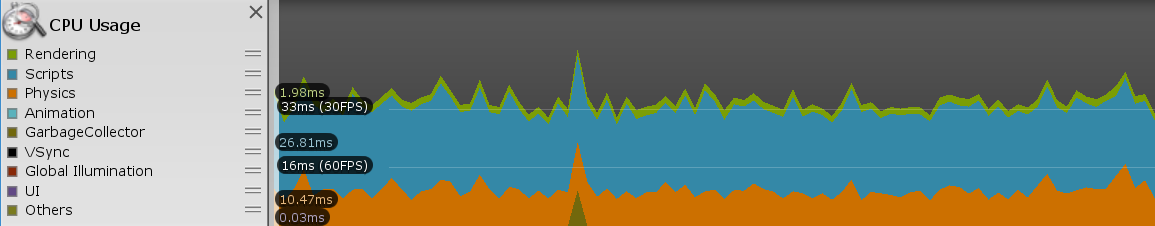
\includegraphics[width=\textwidth]{pictures/profiling.png}
		\caption{CPU utilization output from Unity's Profiler}
		\label{fig:unity:profiler}
	\end{figure}
\end{frame}

\begin{frame}{\secname}{\subsecname}
	Experience with Unity C\# Job System
	\begin{itemize}
		\item (Almost) writing C++ in C\#
		\begin{itemize}
			\item Manually scheduling \texttt{Job}s
			\item Memory leaks if \texttt{NativeContainer}s are not \texttt{Dispose}d
		\end{itemize}
		\item No simple way of handling dependencies between \texttt{JobSystem}s
		\item A lot of converting between representations
		\item Some expensive operations, such as \texttt{Instantiate} must happen on main thread
		\item \textbf{A lot of effort for no/limited performance gain}
	\end{itemize}
\end{frame}

\section{Usability Findings}
\begin{frame}{\secname}{Disposition}
	Usability findings in the project.
	\begin{itemize}
		\item<2-> High Perceived Cost
		\item<3-> Cultural Shock
		\item<4-> Difference of Priority
	\end{itemize}
\end{frame}

\subsection{High Perceived Cost}
\begin{frame}{\secname}{\subsecname}
	\fs considered costly and harmful to productivity.
	\begin{itemize}
		\item<2-> Productivity Cost
		\item<3-> Popularity
		\item<4-> Ease of Use
	\end{itemize}
\end{frame}

\subsection{Cultural Shock}
\begin{frame}{\secname}{\subsecname}
	Idiomatic barriers between \cs and \fs.
	\begin{itemize}
		\item<2-> Traditionally Object Oriented
		\item<3-> Functional Paradigm
		\item<4-> Higher Level of Abstraction
	\end{itemize}
\end{frame}

\subsection{Difference of Priority}
\begin{frame}{\secname}{\subsecname}
	Dissonance between our expectations and that of the developers.
	\begin{itemize}
		\item<2-> Maintainability is low priority
		\item<3-> Code quality was not a priority
		\item<4-> \dquote{\textit{Productivity is King}}
	\end{itemize}
\end{frame}

\section{Coginitive Dimensions Analysis}
\begin{frame}{\secname}{Disposition}
	Notable Instances
	\begin{itemize}
		\item Abstraction Gradient
		\item Closeness of Mapping
		\item Consistency
		\item Error-proneness
		\item Hard Mental Operations
		\item Progressive Evaluation
		\item Role-expressiveness
	\end{itemize}
\end{frame}

\subsection{Abstraction Gradient}
\begin{frame}{\secname}{\subsecname}
	Closer to C++
	\begin{itemize}
		\item Unity imposes lower level of Abstraction
	\end{itemize}
\end{frame}

\subsection{Closeness of Mapping}
\begin{frame}{\secname}{\subsecname}
	Departure from Composite Pattern
	\begin{itemize}
		\item Scene behaviour vs. Management Object Singleton
		\item Object properties on system instead of object
		\begin{itemize}
			\item System controls object target
		\end{itemize}
	\end{itemize}
\end{frame}

\subsection{Consistency}
\begin{frame}{\secname}{\subsecname}
	Unexpected Features
	\begin{itemize}
		\item \m{NativeArray}
		\begin{itemize}
			\item Requires non-nullable type
			\item Cannot be extended
			\item Requires manual memory management
		\end{itemize}
		\item \m{TransformAccess} does not have the same methods as \m{Transform}
		\item \m{UnityEngine.Random.Range} can only be called on the main thread
	\end{itemize}
\end{frame}

\subsection{Error-proneness}
\begin{frame}{\secname}{\subsecname}
	Sources of Problems
	\begin{itemize}
		\item Job Scheduling
		\item Ideal code structure is not obvious
	\end{itemize}
\end{frame}

\subsection{Hard Mental Operations}
\begin{frame}{\secname}{\subsecname}
	Mental Tongue Twisters
	\begin{itemize}
		\item Manual vector calculation
		\item Dependency determination
		\item Job management
		\begin{itemize}
			\item Job responsibility
			\item System responsibility
		\end{itemize}
		\item Memory management
	\end{itemize}
\end{frame}

\subsection{Progressive Evaluation}
\begin{frame}{\secname}{\subsecname}
	The Editor
	\begin{itemize}
		\item Editor Errors
		\begin{itemize}
			\item Exceptions carry over from previous runs
			\item Requires restart
		\end{itemize}
		\item Editor Crashes
	\end{itemize}
\end{frame}

\subsection{Role-expressiveness}
\begin{frame}{\secname}{\subsecname}
	Breaking from Convention
	\begin{itemize}
		\item Nonconventional names
		\begin{itemize}
			\item \m{NativeContainer} should be \m{NativeCollection}
			\item \m{System} is a vague name
		\end{itemize}
	\end{itemize}
\end{frame}

\section{Attention Investment}
\begin{frame}{\secname}{\subsecname}
	Attention Investment Metrics
	\begin{itemize}
		\item Cost
		\item Investment
		\item Pay-off
		\item Risk
	\end{itemize}
\end{frame}

\subsection{Cost}
\begin{frame}{\secname}{\subsecname}
	Cost
	\begin{itemize}
		\item Lower abstraction (closer to machine)
		\item Scheduling
		\item Division of work
		\item Additional management systems
	\end{itemize}
\end{frame}

\subsection{Investment}
\begin{frame}{\secname}{\subsecname}
	Investment
	\begin{itemize}
		\item Schedule understanding
		\item Objects into systems
	\end{itemize}
\end{frame}

\subsection{Pay-off}
\begin{frame}{\secname}{\subsecname}
	Pay-off
	\begin{itemize}
		\item Increased performance
		\item Greater resource utilisation
	\end{itemize}
\end{frame}

\subsection{Risk}
\begin{frame}{\secname}{\subsecname}
	Risk
	\begin{itemize}
		\item No pay-off
		\item Error introduction
		\begin{itemize}
			\item Memory leaks
		\end{itemize}
		\item Failed implementation
	\end{itemize}
\end{frame}

\section{Future Work}
\begin{frame}{\secname}{Disposition}
	Research Topics
	\begin{itemize}
		\item Gameplay Programming vs. Engine Programming
		\item Imperative vs. Object Oriented Conflict
	\end{itemize}
\end{frame}

\subsection{Gameplay Programming vs. Engine Programming}
\begin{frame}{\secname}{\subsecname}
	Different Priorities
	\begin{itemize}
		\item Responsible for performance
		\item Engine life time
		\item Architecture
	\end{itemize}
\end{frame}

\subsection{Imperative vs. Object Oriented Conflict}
\begin{frame}{\secname}{\subsecname}
	Separate Conflict
	\begin{itemize}
		\item Runtime Coupling
		\item C++ vs. C#
		\item JIT vs. AOT
	\end{itemize}
\end{frame}


\begin{frame}{References}
  \printbibliography
\end{frame}

{\aauwavesbg
\begin{frame}[plain,noframenumbering]
  \finalpage{Thank you for your attention}
\end{frame}}

\end{document}
